\documentclass[english,10pt,aspectratio=169]{beamer}

\usepackage{amsmath} % load this before unicode-math
\usepackage{amssymb}
%\usepackage{unicode-math}

\usepackage{fontspec}
\setmonofont{JuliaMono}

\usefonttheme[onlymath]{serif}

\setlength{\parskip}{\smallskipamount}
\setlength{\parindent}{0pt}

%\setbeamersize{text margin left=5pt, text margin right=5pt}

\usepackage{amsmath}
\usepackage{amssymb}
\usepackage{braket}
\usepackage{mhchem}

\usepackage{minted}
\newminted{julia}{breaklines,fontsize=\scriptsize,texcomments=true}
\newminted{python}{breaklines,fontsize=\scriptsize,texcomments=true}
\newminted{bash}{breaklines,fontsize=\scriptsize,texcomments=true}
\newminted{text}{breaklines,fontsize=\scriptsize,texcomments=true}

\newcommand{\txtinline}[1]{\mintinline[fontsize=\scriptsize]{text}{#1}}
\newcommand{\jlinline}[1]{\mintinline[fontsize=\scriptsize]{julia}{#1}}

\definecolor{mintedbg}{rgb}{0.95,0.95,0.95}
\usepackage{mdframed}

%\BeforeBeginEnvironment{minted}{\begin{mdframed}[backgroundcolor=mintedbg]}
%\AfterEndEnvironment{minted}{\end{mdframed}}

\setcounter{secnumdepth}{3}
\setcounter{tocdepth}{3}

\makeatletter

 \newcommand\makebeamertitle{\frame{\maketitle}}%
 % (ERT) argument for the TOC
 \AtBeginDocument{%
   \let\origtableofcontents=\tableofcontents
   \def\tableofcontents{\@ifnextchar[{\origtableofcontents}{\gobbletableofcontents}}
   \def\gobbletableofcontents#1{\origtableofcontents}
 }

\makeatother

\usepackage{babel}

\begin{document}


\title{Recent CMD ITB Lab Research on\\
Density Functional Theory Software Development}
\author{Fadjar Fathurrahman}
\institute{
Engineering Physics \\
Institut Teknologi Bandung
}
\date{24 February 2022}

\frame{\titlepage}


\begin{frame}[fragile]
\frametitle{Some background information}

My first exposure to first-principles calculations (around 2008-2010):
\begin{itemize}
\item ABINIT, CPMD, Quantum Espresso, PyQuante, ELK, ...
\item Asian CMD Workshop
\item Learning Linux environment
  \begin{itemize}
  \item Using compilers, \txtinline{configure}, \txtinline{make}, \txtinline{make install}
  \item Linking to libraries: BLAS, LAPACK
  \end{itemize}
\end{itemize}

I use Quantum Espresso for my bachelor thesis.

%Learn DFT by using the softwares to do the calculations.
%I am still learning by now

\end{frame}



\begin{frame}
\frametitle{Course about DFT in TF ITB (2010)}

\begin{itemize}
\item Taught by Prof. Hermawan. Based on Prof. Arias course materials:
  \begin{itemize}
  \item Old website: {\footnotesize\url{https://dft.physics.cornell.edu/old-website/minicourse/}}
  \item New website: {\footnotesize\url{http://jdftx.org/PracticalDFT.html}}
  \end{itemize}
\item Using C programming language and Octave (a MATLAB clone)
\item Plane wave basis set and DFT++ formalism
\item Problems:
  \begin{itemize}
  \item radial atomic problem
  \item quantum dot (with harmonic potential confinement)
  \item H atom $\ce{H2}$ molecule in a box
  \item Ge crystal (8 atoms in a cubic unit cell, local pseudopotential)
  \end{itemize}
\item Only local pseudopotentials (available only to some elements), no $\mathbf{k}$-points
\item DFT++ formalism is not widely adopted in the literature
\end{itemize}

\end{frame}


\begin{frame}
\frametitle{First try: plane wave pseudopotential code (2010-2012)}

\begin{itemize}
\item During my master thesis, I decided to write my own density functional theory
based on plane wave and pseudopotential (parallelized on GPU using CUDA):
{\footnotesize\url{https://github.com/f-fathurrahman/ffr-pspw-dft-c}} \\
WARNING: Not maintained anymore.
\item Motivation:
  \begin{itemize}
  \item Only requires a laptop (two core, 1 GB memory)
  \item What are actually calculated by the DFT packages?
  \item Learn by doing: how DFT or Kohn-Sham equations are solved (beyond described in
  textbooks or research papers)
  \item Sometimes pseudocode is not enough
  \end{itemize}
\item Based on \txtinline{FHI98md} code (originally written in Fortran 77 with  F90 extension).
\end{itemize}

\end{frame}


\begin{frame}
\frametitle{Programming languages for DFT (solid-state)}
    
Programming languages used:
\begin{itemize}
\item Fortran (mostly): ABINIT, VASP, Quantum Espresso, CP2K, ELK, ...
\item C/C++ (mostly): JDFTX, OPENMX, QBOX, ...
\item Python (computationally heavy parts are implemented in C/C++/Fortran): GPAW, QuantumATK (VNL), ...
\item MATLAB: KSSOLV, RESCU, MSPARC, ...
\end{itemize}
    
Static languages: Fortran, C/C++

Dynamic languages: Python, MATLAB

\end{frame}


\begin{frame}
\frametitle{Second try (2015-2018)}

Mostly using Fortran:
\begin{itemize}
\item {\footnotesize\url{https://github.com/f-fathurrahman/ffr-LFDFT}} (Lagrange basis functions)
\item {\footnotesize\url{https://github.com/f-fathurrahman/ffr-PWDFT}} (plane wave basis functions)
\end{itemize}

Not in active development

\end{frame}



\begin{frame}
\frametitle{Latest try (2015-now): PWDFT.jl}

{\footnotesize\url{https://github.com/f-fathurrahman/PWDFT.jl}}

{\footnotesize\url{https://doi.org/10.1016/j.cpc.2020.107372}} (still 0 citation)

{\centering
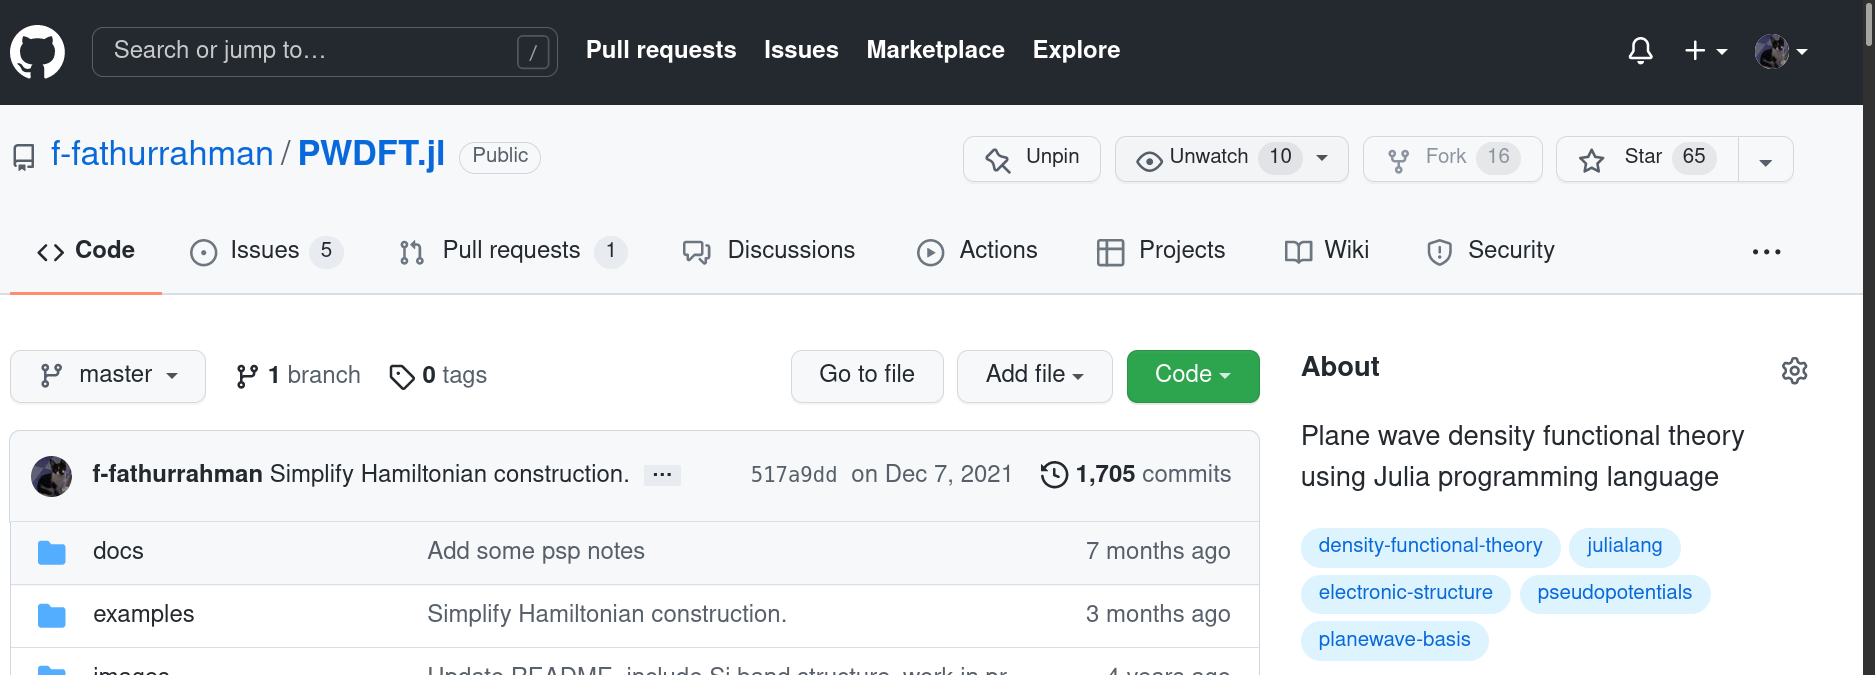
\includegraphics[width=\textwidth]{images/PWDFT_github.png}
\par}

\end{frame}


\begin{frame}
\frametitle{Some features}

{\centering

\includegraphics[width=0.20\textwidth]{images/julia_logo_v1.pdf}
\par}

\begin{itemize}
\item Implemented in Julia programming language {\footnotesize \url{https://julialang.org/}}
\item Plane wave basis and norm-conserving pseudopotentials (mostly with
Goedecker-Teter-Hutter pseudopotentials, ONCV)
\item $\mathbf{k}$-points sampling
\item Currently only periodic boundary condition
\item total energy and atomic forces
\item LDA (VWN), GGA (PBE), and metaGGA (SCAN) via Libxc
\item Does not require specific input file format, we write a Julia
script instead
\end{itemize}

\end{frame}


\begin{frame}
\frametitle{Julia programming language}

Some pros:
\begin{itemize}
\item A rather new programming language (2009, announced 2012), first developed by
Jeff Bezanson, Stefan Karpinski, Viral B. Shah, and Alan Edelman.
\item The syntax is familiar to MATLAB or Python users
\item Built-in support for multidimensional array and linear algebra
(like MATLAB and Fortran)
\item Loop is fast, no need for vectorization (as in other ecosystems or
programming languages like MATLAB, Python (Numpy), or R)
\end{itemize}

Some cons:
\begin{itemize}
\item Large runtime (LLVM, OS specific functions, garbage collectors, ...)
\item Compilation time (e.g. time-to-first-plot problem)
\item No straighforward way to produce single executable file
\item Smaller community (compared to Python, MATLAB, R, etc)
\end{itemize}


\end{frame}




\begin{frame}
\frametitle{Aims of PWDFT.jl}

\begin{itemize}
\item Friendly-to-developers DFT package: enables quick implementation of various algorithms
\item Educational purpose: simple yet powerful enough to carry out practical DFT calculations
for molecular and crystalline systems.
\end{itemize}

\textsf{PWDFT.jl} is not intended to be a replacement for other well-established
DFT softwares.

\end{frame}

\begin{frame}[fragile]
\frametitle{Example: hydrogen molecule in a box}

{\centering
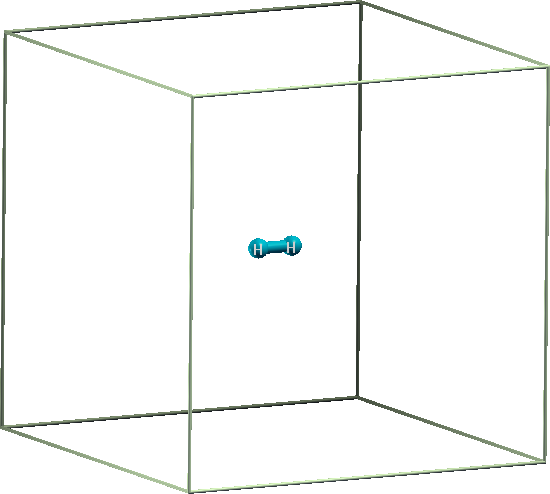
\includegraphics[width=0.20\textwidth]{images/H2.png}
\par}

\begin{juliacode}
using PWDFT # activate PWDFT package

# Initialize an H2 molecule in cubic box (simple cubic lattice)
# The coordinates are read from
atoms = Atoms( xyz_file="H2.xyz",
               LatVecs=gen_lattice_sc(16.0) )

pspfiles = ["H-q1.gth"] # pseudopotential parameters

ecutwfc = 15.0 # cutoff energy for wave function expansion

# initialize Hamiltonian
Ham = Hamiltonian( atoms, pspfiles, ecutwfc )

# solve the Kohn-Sham problem (using SCF algorithm)
KS_solve_SCF!( Ham )
\end{juliacode}

\end{frame}



%--------------------------------------------------------------
\begin{frame}
\frametitle{Status}
  
{\centering
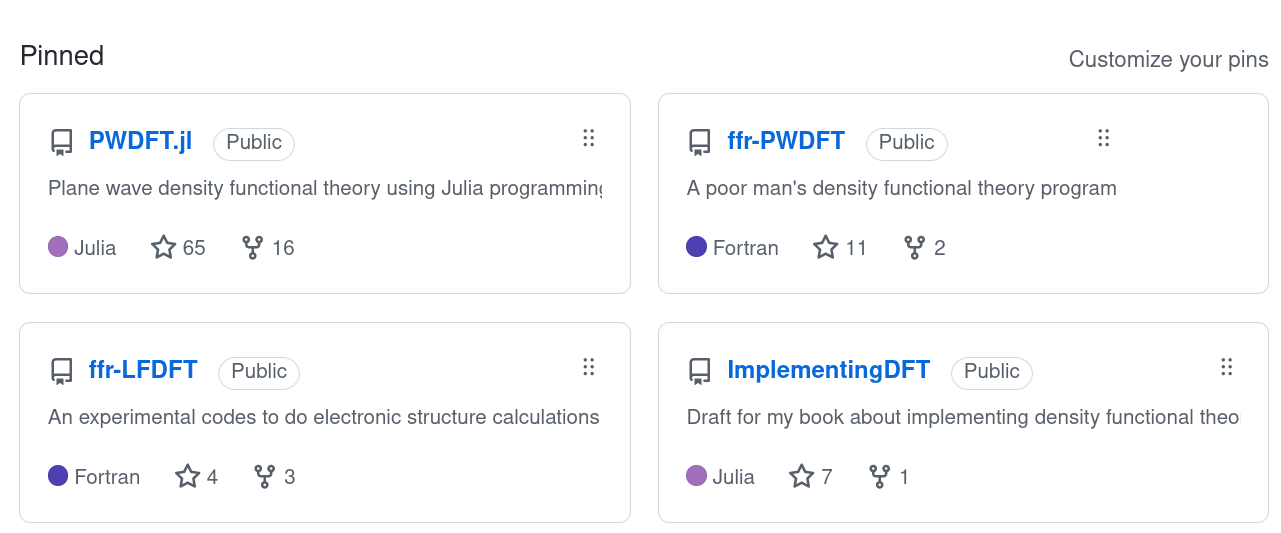
\includegraphics[width=\textwidth]{images/Github_ffr.png}
\par}

\end{frame}


%--------------------------------------------------------------
\begin{frame}
\frametitle{Wikipedia citation}

{\centering
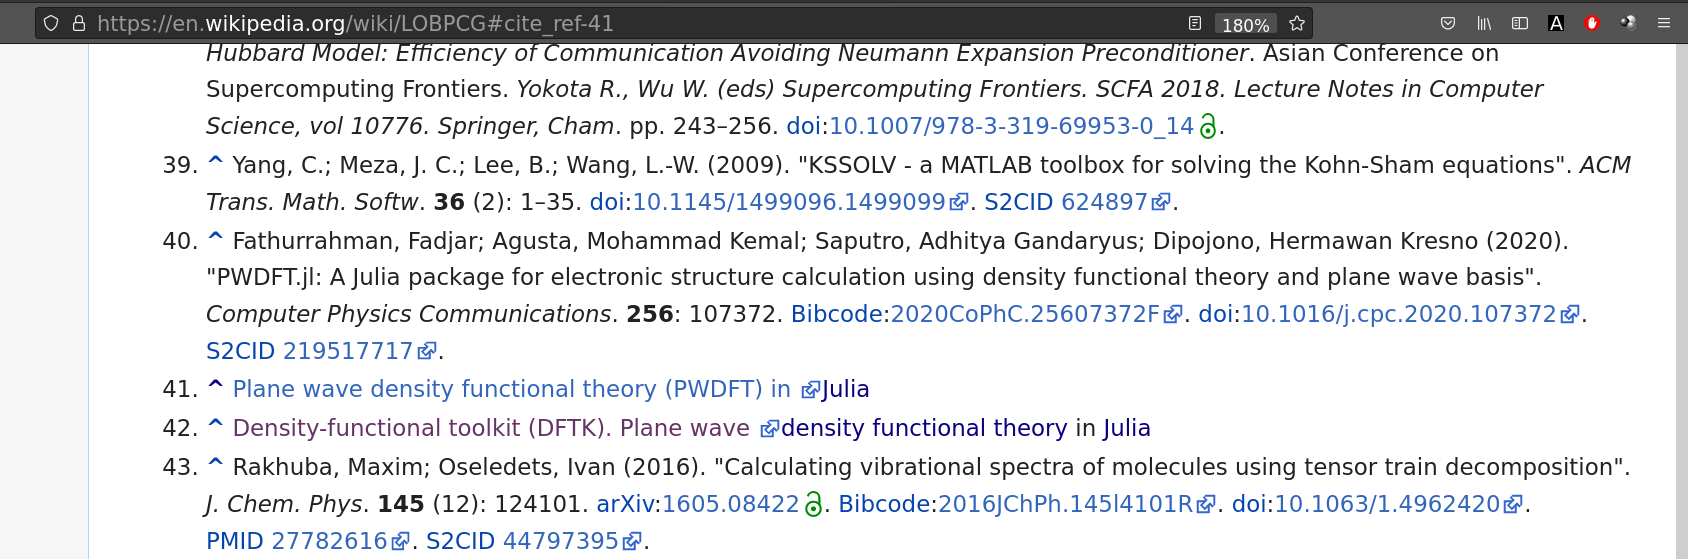
\includegraphics[width=\textwidth]{images/LOBPCG_wikipedia.png}
\par}

{\footnotesize
\url{https://en.wikipedia.org/wiki/LOBPCG\#cite_note-40}
}

\end{frame}


%--------------------------------------------------------------
\begin{frame}
\frametitle{Twitter mentions}

{\centering
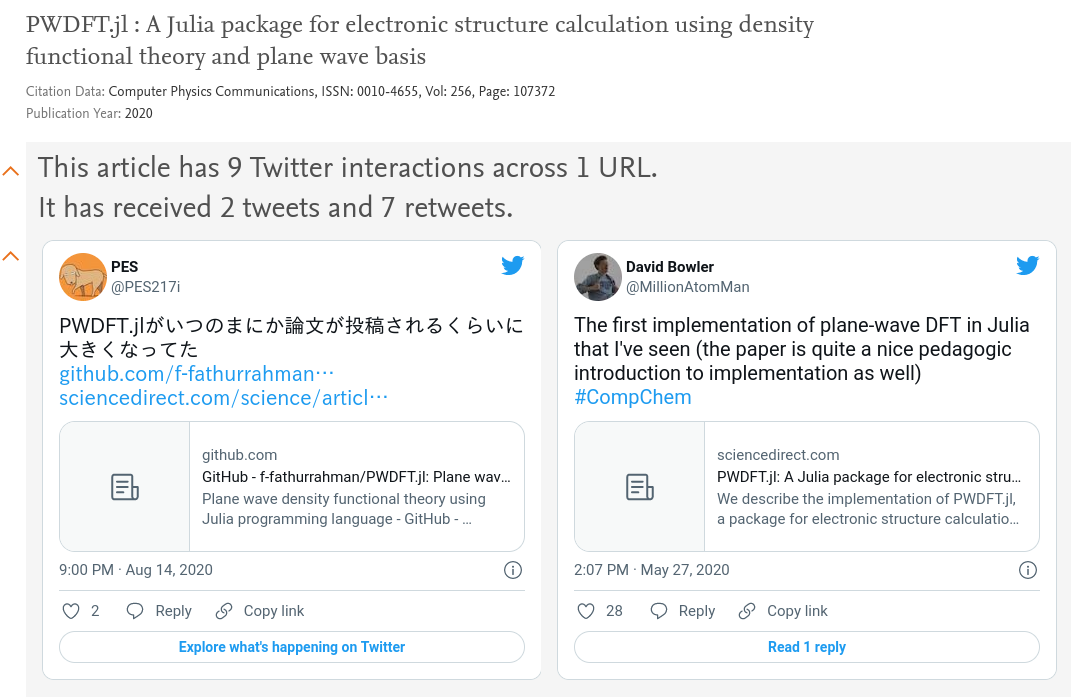
\includegraphics[width=0.7\textwidth]{images/Plumx_Tweet.png}
\par}

{\footnotesize
\url{https://plu.mx/plum/a/twitter?doi=10.1016/j.cpc.2020.107372}
}

\end{frame}


\begin{frame}
\frametitle{Many things are still to be done}

\begin{itemize}
\item documentation, unit testing, 
\item maintenance, bug fixes, 
\item implement new features:
  \begin{itemize}
  \item performance improvement
  \item ultrasoft and PAW
  \item parallelization
  \item on-the-fly atomistic machine learning potential generation
  \item machine-learning-fitted exchange correlation potential
  \item Export KS orbitals to QMC (?), write a simple QMC code (?)
  \item ...
  \end{itemize}
\end{itemize}

\end{frame}


\end{document}

